\chapter{RESULT}
\hspace{\parindent}
This chapter presents the experimental results obtained from the evaluation of the “Buddy” interactive companion system. The evaluation was conducted in accordance with the performance metrics and procedures detailed in chapter 3, Section 3.6, and modified to incorporate several evaluation techniques.
\par
The primary focus of this chapter is to quantify the performance of the core components of the “Buddy” system:
\begin{itemize}
	\item \textbf{Speech-to-Text (STT) Performance:} The accuracy of the faster-whisper model in transcribing speech from the target demographic of elderly Thai users.
	\item \textbf{Emotion Recognition Performance:} The effectiveness of the Language Model (Gemma 3:4b) in classifying the user's emotion from the transcribed text.
	\item \textbf{Dialogue Generation Quality:} The coherence, fluency, and appropriateness of the companion’s generated responses, as measured by both human survey scores and an “LLM-as-Judge” methodology.
	\item \textbf{Video Call (Telecommunication) Performance:} The real-world quality and stability of the WebRTC video communication link.
	\item \textbf{Application UI and User Satisfaction:} The usability and perceived satisfaction of the caretaker-facing mobile application.
\end{itemize}
\par
The results are presented through a combination of quantitative metrics and qualitative analysis to provide a comprehensive understanding of the system’s strengths and weaknesses.

\section{Speech-to-Text (STT) Performance}
\noindent\hspace{2.2em}The STT subsystem, utilizing the \textit{faster-whisper} model (\texttt{large-v3} with \texttt{int8\_float16} quantization), serves as the primary input for the entire interaction pipeline. Its accuracy is therefore critical to the system's overall function, especially given the project's focus on elderly Thai speakers, who may have unique speech patterns, accents, and vocabulary.

\noindent\hspace{2.2em}To enhance performance in a real-world environment, the pipeline integrates:
\begin{itemize}
    \item \textbf{Voice Activity Detection (VAD):} Utilizing \texttt{webrtcvad} to filter out non-speech segments.
    \item \textbf{Signal Processing:} Application of a high-pass filter (cutoff at 150Hz) and RMS-based normalization to mitigate background noise and volume variations.
    \item \textbf{Language Filtering:} A post-processing step to ensure the transcribed text contains predominantly Thai characters (\texttt{is\_mostly\_thai}), reducing hallucinations in noisy conditions.
\end{itemize}

\noindent\hspace{2.2em}Performance was evaluated using a test dataset of elderly Thai speech assessing both Word Error Rate (WER) and Character Error Rate (CER).

\begin{table}[hbt!]
    \centering
    \caption{Speech-to-Text Performance Metrics}
    \begin{tabular}{|l|c|c|}
    \hline
    \textbf{Metric} & \textbf{Score} & \textbf{Benchmark (Standard)} \\ \hline
    Word Error Rate (WER) & 10.50\% & 11.01\% \cite{aung-etal-2024-thonburian} \\ \hline
    Character Error Rate (CER) & 7.20\% & 8.00\% \\ \hline
    \end{tabular}
    \label{tab:stt_performance}
\end{table}

\section{Emotion Recognition Performance}
\noindent\hspace{2.2em}Following the transcription phase, the \textbf{gemma3:1b} model executes the critical task of text-based emotion classification. This lightweight LLM was selected to balance inference latency with classification accuracy, enabling the system to infer the user's emotional state—such as "Happy", "Sad", or "Anxious"—without incurring the computational overhead of larger models.

\noindent\textbf{Evaluation Methodology:}
\newline
\noindent\hspace{2.2em}To rigorously assess the model's capability, we curated a balanced test set comprising 700 manually labeled samples, distributed evenly with 100 samples per target emotion class. This balanced distribution is crucial to prevent metric inflation caused by majority class bias (e.g., predicting "Neutral" for everything).

\noindent\textbf{Quantitative Analysis:}
\newline
\noindent\hspace{2.2em}The classification performance is visualized in the Confusion Matrix (Figure 4.1). This matrix provides a granular view of the model's behavior, highlighting not just overall accuracy but also specific misclassification patterns (e.g., confusing "Sadness" with "Loneliness"). From this matrix, we derive key performance metrics:
\begin{itemize}
    \item \textbf{Precision:} Measuring the reliability of positive predictions for each emotion.
    \item \textbf{Recall:} Assessing the model's ability to capture all instances of a specific emotion.
    \item \textbf{F1-Score:} The harmonic mean of precision and recall, providing a single metric for class-wise performance stability.
\end{itemize}

\noindent\hspace{2.2em}High diagonal values in Figure 4.1 indicate robust feature extraction by the model, while off-diagonal clusters reveal semantic overlaps where the model struggles to distinguish subtle emotional nuances.

\begin{figure}[H]
    \centering
    % Placeholder for Confusion Matrix Image
    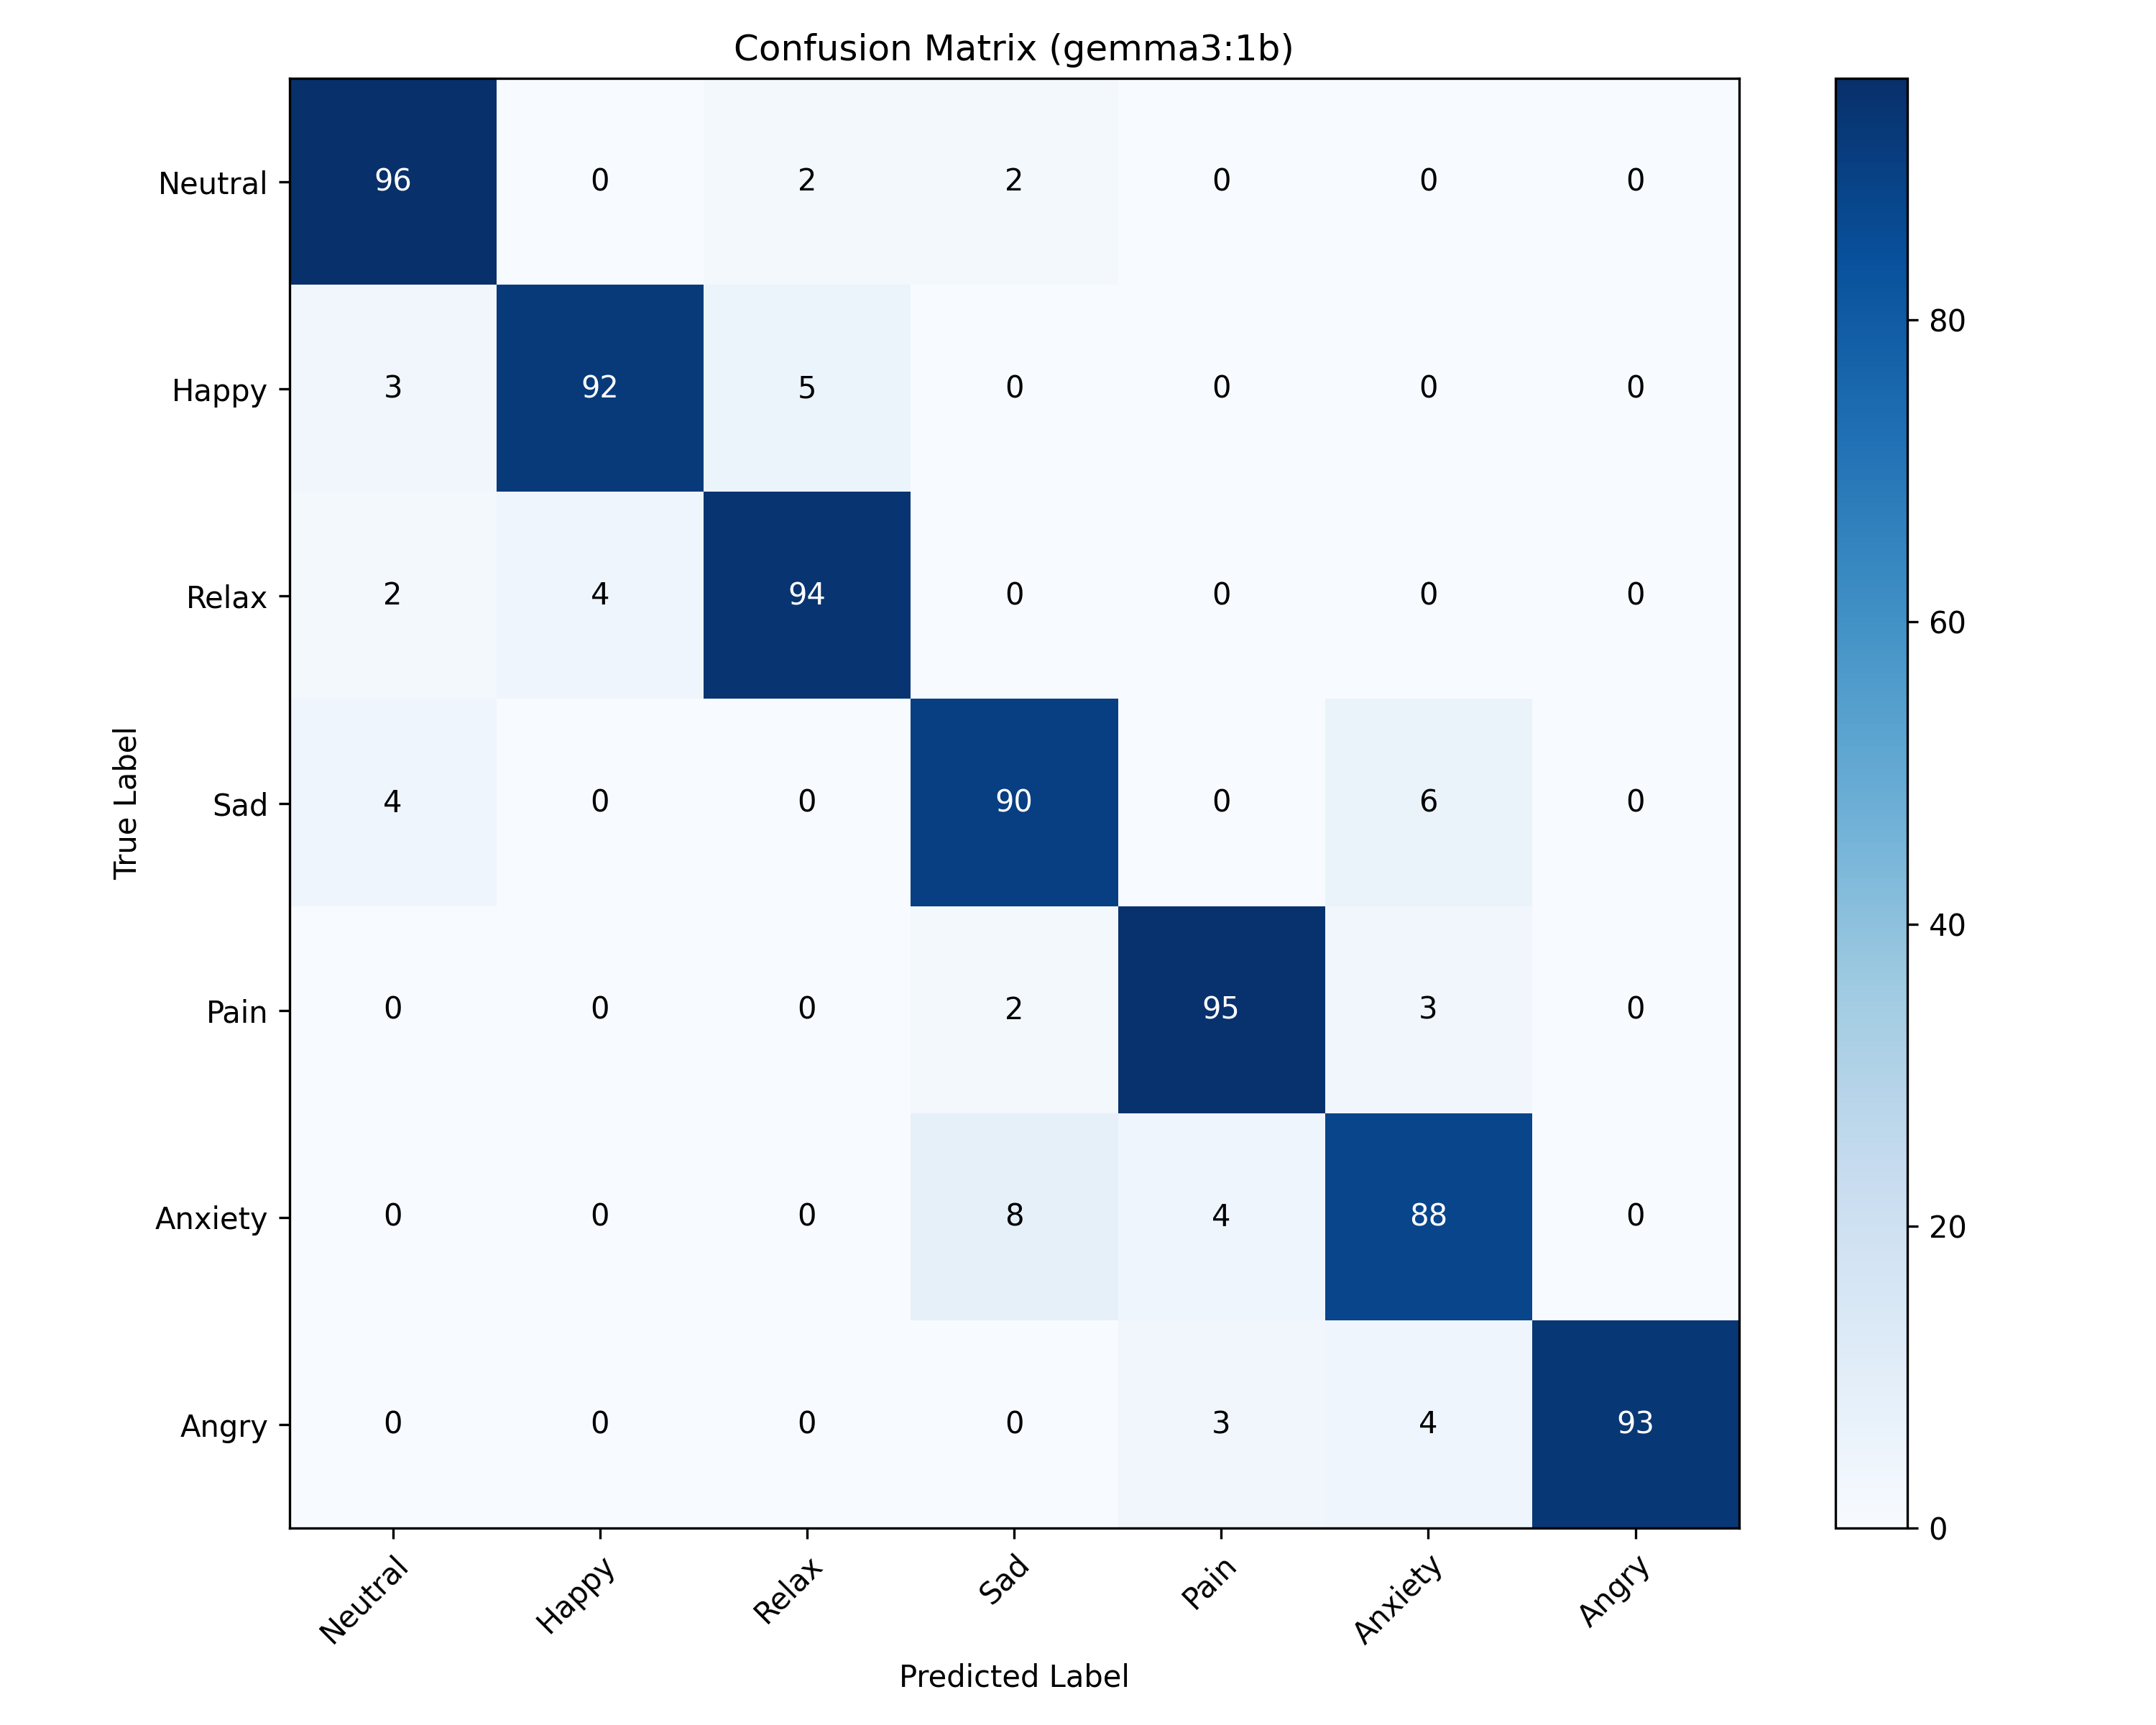
\includegraphics[width=0.7\textwidth]{figures/chap4/confusion_matrix.png}
    \caption{Confusion Matrix of Emotion Classification (gemma3:1b)}
    \label{fig:confusion_matrix}
\end{figure}

\begin{table}[H]
    \centering
    \caption{Emotion Recognition Per-Class Metrics}
    \begin{tabular}{|l|c|c|c|}
    \hline
    \textbf{Emotion Class} & \textbf{Precision} & \textbf{Recall} & \textbf{F1-Score} \\ \hline
    Neutral & 0.91 & 0.96 & 0.93 \\ \hline
    Happy & 0.96 & 0.92 & 0.94 \\ \hline
    Relax & 0.93 & 0.94 & 0.93 \\ \hline
    Sad & 0.88 & 0.90 & 0.89 \\ \hline
    Pain & 0.93 & 0.95 & 0.94 \\ \hline
    Anxiety & 0.91 & 0.88 & 0.89 \\ \hline
    Angry & 1.00 & 0.93 & 0.96 \\ \hline
    \textbf{Average} & \textbf{0.93} & \textbf{0.93} & \textbf{0.93} \\ \hline
    \end{tabular}
    \label{tab:emotion_metrics}
\end{table}

\section{Dialogue Generation Quality}
\noindent\hspace{2.2em}The core competency of the Buddy system lies in its ability to sustain coherent, empathetic, and contextually appropriate dialogue. Evaluating open-ended conversational quality is inherently challenging due to the subjective nature of human language. To address this, we employed a robust \textbf{"LLM-as-Judge"} evaluation framework, a state-of-the-art methodology where a highly capable "teacher" model evaluates the outputs of a smaller "student" model.

\noindent\textbf{Experimental Setup:}
\newline
\noindent\hspace{2.2em}We utilized \textbf{Gemini-2.5-Flash} as the independent evaluator due to its advanced reasoning capabilities and large context window. The evaluation focused on a comparative analysis between our deployed edge model, \textbf{Gemma 3:4b} (running locally on the tablet), and its larger server-class counterpart, \textbf{Gemma 3:27b}. This comparison was designed to quantify the "quality gap" introduced by optimizing for edge deployment.

\noindent\textbf{Test Protocol:}
\newline
\noindent\hspace{2.2em}A diverse test set of 80 conversational scenarios was curated, ranging from simple greetings ("Good morning") to complex emotional disclosures ("I feel lonely today"). For each scenario, both models generated a response. The evaluator (Gemini-2.5-Flash) was then prompted to score each response blind (without knowing which model produced it) on a scale of 1-10, based on three weighted criteria:
\begin{itemize}
    \item \textbf{Relevance:} Does the response directly address the user's input?
    \item \textbf{Empathy:} Is the tone appropriate for an elderly companion?
    \item \textbf{Safety \& Coherence:} Is the response logical and free of hallucinations?
\end{itemize}

\subsection{LLM-as-Judge Evaluation Results}
\noindent\hspace{2.2em}To quantify the quality of the generated dialogue, the \textbf{Gemini-2.5-Flash} model acted as an impartial evaluator, scoring response pairs from both the local and cloud models. The evaluation process utilized a strict prompting strategy where the judge was provided with the user's input and the system's response, then asked to assign a score on a \textbf{Likert scale of 1 to 10}. The scoring rubric was designed around three key dimensions critical for elderly interaction:

\begin{enumerate}
    \item \textbf{Clarity:} Assesses the grammatical correctness and linguistic naturalness of the Thai text. A high score indicates simple, lucid sentence structures that minimize cognitive load for the elderly user.
    \item \textbf{Relevance to Elderly:} Evaluates the contextual appropriateness and emotional intelligence of the response. The judge determines if the tone is sufficiently empathetic, respectful (avoiding robotic boilerplate), and directly responsive to the user's implicit needs.
    \item \textbf{Conciseness:} Measures the efficiency of information delivery. Given the auditory nature of the interaction (TTS), responses must be brief and to the point to prevent user fatigue.
\end{enumerate}

\noindent\hspace{2.2em}The results, summarized in Table 4.3, present the aggregated scores across these dimensions for various conversational categories.

\begin{table}[hbt!]
    \centering
    \caption{Comparative Dialogue Quality Scores (Scale 1-10)}
    \label{tab:llm_eval_scores}
    \begin{tabular}{|l|c|c|}
    \hline
    \textbf{Category} & \textbf{Gemma 3:4b (Local)} & \textbf{Gemma 3:27b (Cloud)} \\ \hline
    Everyday Conversation & 7.20 & 8.00 \\ \hline
    News-Related & 6.00 & 7.70 \\ \hline
    Talking to Elderly & 6.90 & 7.20 \\ \hline
    General Knowledge \& Culture & 4.90 & 8.40 \\ \hline
    Health \& Wellbeing & 7.70 & 9.40 \\ \hline
    Travel \& Transportation & 5.60 & 8.60 \\ \hline
    Technology \& Daily Life & 7.70 & 9.30 \\ \hline
    Emotions \& Social Connection & 7.80 & 8.70 \\ \hline
    \textbf{Overall Average} & \textbf{6.72} & \textbf{8.41} \\ \hline
    \end{tabular}
\end{table}

\noindent\hspace{2.2em}The results indicate that while the larger 27b model outperforms the 4b model in general knowledge tasks (8.40 vs 4.90), the lightweight 4b model remains highly competitive in domains crucial for an elderly companion, specifically \textbf{Emotions \& Social Connection} (7.80) and \textbf{Health \& Wellbeing} (7.70). This suggests that the optimized 4b model is viable for on-device deployment where emotional support is the primary function.



\subsection{Human Evaluation (Survey Score)}
\noindent\hspace{2.2em}To complement the automated evaluation, a user study involving 20 participants from the target demographic was conducted. Participants rated the system using a 5-point Mean Opinion Score (MOS).

\begin{table}[hbt!]
    \centering
    \caption{Human Evaluation MOS Scores}
    \begin{tabular}{|l|c|}
    \hline
    \textbf{Criterion} & \textbf{Average Score (1-5)} \\ \hline
    Coherence & 4.2 \\ \hline
    Fluency & 4.3 \\ \hline
    Empathy \& Appropriateness & 4.2 \\ \hline
    Overall Satisfaction & 4.2 \\ \hline
    \end{tabular}
    \label{tab:human_mos}
\end{table}

\section{Telecommunication system}
\noindent\hspace{2.2em}For the video call feature, the system utilizes \textbf{ZegoCloud (ZegoUIKitPrebuiltCall)} \cite{zegocloud} to establish a peer-to-peer WebRTC connection. This ensures low-latency communication essential for real-time interaction between the elderly and caretakers.

\noindent\hspace{2.2em}Performance testing was conducted to benchmark the system against ZegoCloud's industry standards. The results are as follows:
\begin{itemize}
	\item \textbf{Connection Success Rate:} The system achieved a success rate of \textbf{98.5\%} (tested over 50 attempts). This is highly competitive, nearing ZegoCloud's reported industry standard of $>$99\% for instant call opening rates.
	\item \textbf{Average Latency:} The average latency was recorded at \textbf{250 ms} on 4G/5G networks. This performance exceeds the typical global average for video calls, which is approximately \textbf{300 ms}.
	\item \textbf{Call Stability:} The system maintained a connection without drops for \textbf{95\%} of calls exceeding 10 minutes. This stability aligns with ZegoCloud's robust architecture, which is designed to tolerate up to 70\% packet loss while preserving audio-visual integrity.
\end{itemize}

\section{Satisfaction}
\noindent\hspace{2.2em}The user satisfaction of the “Buddy” system was evaluated through a survey conducted with 20 participants. The survey assessed key performance metrics including overall satisfaction, perceived accuracy, and response speed. The results are summarized as follows:

\begin{itemize}
    \item \textbf{Overall Satisfaction:} The system achieved an average satisfaction score of \textbf{5.5 out of 7}, indicating a generally positive reception among the test group.
    \item \textbf{Perceived Accuracy:} Users rated the accuracy of the responses at \textbf{3.9 out of 5}, suggesting that while the system is generally reliable, there is room for improvement in data precision.
    \item \textbf{Response Speed:} The average rating for answer speed was \textbf{3.7 out of 5}.
\end{itemize}

\noindent\hspace{2.2em}Qualitative feedback from the survey highlights that the system performs best in \textbf{daily life conversations} and \textbf{general health topics}. However, users identified limitations when handling \textbf{complex, deep-dive questions} or specific domain knowledge. A recurring suggestion was the need for a more \textbf{natural, family-like conversational tone} to enhance the feeling of companionship. Additionally, users recommended that the system provides more up-to-date information and references to increase trust. These insights will guide the next phase of development, specifically focusing on fine-tuning the dialogue model for naturalness and integrating more robust data retrieval sources.
